% SPDX-License-Identifier: CC-BY-4.0
% Copyright (c) 2026 Martin Schröder <info@swedishembedded.com>
%
% Swedish Embedded AB implements autonomous fine-tuning and held-out
% evaluation of language models for its clients. If your team needs expertise
% in training a model from a body of text and measuring, with honest
% statistics, whether it learned anything, you can procure our services by
% sending an email to info@swedishembedded.com.

\documentclass[11pt,a4paper]{article}

\usepackage[utf8]{inputenc}
\usepackage[T1]{fontenc}
\usepackage{lmodern}
\usepackage[margin=2.5cm]{geometry}
\usepackage{microtype}
\usepackage{booktabs}
\usepackage{array}
\usepackage{enumitem}
\usepackage{xcolor}
\usepackage{amsmath,amssymb}
\usepackage{tikz}
\usetikzlibrary{positioning,arrows.meta,fit,calc}
\usepackage{pgfplots}
\usepgfplotslibrary{groupplots}
\pgfplotsset{compat=1.17}
\usepackage[numbers,sort&compress]{natbib}
\usepackage{caption}
\usepackage{subcaption}
\usepackage[colorlinks=true,linkcolor=blue!50!black,citecolor=blue!50!black,urlcolor=blue!50!black]{hyperref}
\usepackage[capitalise,nameinlink]{cleveref}

\setlist{nosep,leftmargin=1.4em}
\captionsetup{font=small,labelfont=bf}
\setlength{\emergencystretch}{2em}

\input{generated/macros}

\newcommand{\code}[1]{\texttt{#1}}

\title{Training a Language Model to Think Like a Historical Author\\
from One Sentence and the Author's Own Writings:\\
Pipeline, Evaluation Methodology and an Honest Account of the Results}
\author{Martin Schröder\\
Swedish Embedded AB, \href{mailto:info@swedishembedded.com}{info@swedishembedded.com}}
\date{Working paper, October 2026}

\begin{document}
\maketitle

\begin{abstract}
We describe and evaluate an autonomous pipeline that takes one natural-language
sentence (``Learn to think like \ldots\ based on the materials \ldots\ in directory
\ldots'') and a directory of an author's writings, and produces a LoRA-adapted
language model. The policy is Qwen3-8B in non-thinking mode, an independent Qwen3-14B
is the judge, and all work runs on two 24~GB Tesla P40 GPUs. The pipeline plans,
captures sources, splits them by \emph{family} (all printings of a text), generates and
verifies tasks, teaches, builds a dataset that mixes verified dialogues with the author's
own text, fine-tunes, examines the result on held-out families, and applies a release gate.
Two historical authors, Thomas Jefferson and Samuel Adams, serve as test subjects.

The paper is mainly about method: how such a system is measured, and how its defects were
found and removed. We report the split rule that survives overlapping editions, the
statistical design of an exam that can actually detect an effect, the controls on a
model judge, and a catalogue of defects found by audit: a release gate whose
``held-out'' improvement was paraphrases of trained tasks, a retention check that
failed correct long answers, a monitoring split that silently dropped 27\% of the
author's text, and training-loop mechanics (per-record loss normalisation, a learning
rate that never annealed, weight decay on LoRA, sampling with replacement).

The honest result is negative. On six pilot-scale exams (31--42 tasks, 6--7 families each)
no candidate is statistically distinguishable from the base model told to take the
persona in its prompt at $\alpha=0.05$. Pooled descriptively over four of them, the
adapter judges right on \PooledCandPct\% of tasks against \PooledPromptedPct\% for the
prompted base and \PooledBasePct\% for the unprompted base, and states far fewer
invented specifics than the unprompted base (\PooledCandInv\ against \PooledBaseInv\ of
\PooledTasks\ answers), but those exams have at most about half the power to show even a
very large effect. A frozen 39-family, 244-task exam, whose simulated power for a ten-point
gain is about one half, has been built; its pilot runs had not completed when this paper
was written, and we report them as not measured.
\end{abstract}

% SPDX-License-Identifier: CC-BY-4.0
% Copyright (c) 2026 Martin Schröder <info@swedishembedded.com>

\section{Introduction}\label{sec:intro}

A user who wants a model that reasons and writes ``like'' a historical author
has, today, two cheap options. The first is to tell a general model who to be, in
a system prompt. The second is to fine-tune a model on the author's collected
writings, optionally with synthetic dialogues about them. Whether the second option
buys anything over the first, and how one would know, is the question this paper
studies. We study it inside a concrete system, Splinter, which is given a single
sentence of the form ``Learn to think like \emph{X} based on the materials \emph{X}
has written in directory \emph{D}'' and must, without further instruction, produce a
fine-tuned model together with a measurement of what it learned and a decision on
whether to release it.

We chose two test subjects with large public-domain corpora, Thomas Jefferson (about 1.5
million words of letters and works in the training materials) and Samuel Adams (a smaller
corpus of about one megabyte). The policy is Qwen3-8B~\citep{qwen3} used in non-thinking
mode and adapted with LoRA~\citep{hu2021lora}; the judge is a separate Qwen3-14B. Everything
runs on two Tesla P40 cards with 24~GB each, which constrains the work in ways that shape
the methodology (\cref{sec:residency}).

\paragraph{Scope.}
This paper covers one question: whether fine-tuning a small policy model on one
author's own writings makes it think and write like that author on material it has not
seen, beyond what a persona prompt achieves, and how that is measured. In scope are the
construction of the training data from the author's writings (views, tasks, abstention,
replay), the training mechanics of the adapter, the evaluation design (held-out source
families, exam, judge, statistics, retention), the release gate's checks as measurements,
and the defects in any of these. Out of scope, and reported elsewhere when they have
verified findings of their own, are other uses of the system (timelines and longitudinal
learning, predictive gates, learning from usage policy), retrieval of source passages at
answer time, serving performance, and models other than the Qwen3 pair studied here. A
new finding belongs in this paper if it changes what is claimed about, or how one would
measure, an adapter trained on an author's writings.

\paragraph{The central difficulty is measurement, not training.}
It is easy to produce an adapter that loses a few points of training loss and
sounds a little more archaic. It is hard to show that the adapter has changed what the
model \emph{does} on text it has never seen, beyond what a prompt already achieves, at a
cost to general behaviour that is acceptable. The defects that changed the reported
numbers of the first version of the system were defects of measurement: a split that
leaked, a gate that measured the wrong thing, a grader that failed correct answers, an
exam with too few independent units to detect anything. The training defects were found
by reading the training code, not through the exam numbers.

\paragraph{Contributions.}
\begin{enumerate}
\item A complete, autonomous pipeline from one sentence to a released adapter, with a
  family-level held-out rule that is robust to overlapping editions (\cref{sec:system,sec:split}).
\item An evaluation design for small-corpus persona fine-tuning: an exam reserved
  before any generation, a primary comparison fixed in advance against the
  \emph{persona-prompted} base, per-task pairing with a family-clustered bootstrap, Holm
  correction of secondaries, a power simulation for sizing, and a judge with controls and
  deterministic overrides (\cref{sec:eval}). The design is implemented, its power is
  simulated, four pilot runs on a subset of the exam and full runs of two candidates on all of
  it are reported (\cref{sec:frozen,sec:deployed,sec:full}); the other results of \cref{sec:results} come from an earlier,
  simpler exam (\cref{sec:exam-versions}).
\item A catalogue of defects that were found and fixed, each with the measurement that
  exposed it: leakage across editions, a gate that did not test generalisation, a grader bug,
  the retention suite's inability to detect a two-point drop, and eight training-mechanics
  defects, seven of them corrected (\cref{sec:defects}).
\item Results (\cref{sec:results}). On the earlier exams no candidate is
  distinguishable from the persona-prompted base at $\alpha=0.05$. On the first 25 families
  of the reserved exam, the v7 candidate is not distinguishable from it either (+4.5
  points, family-level $p=0.21$), while the candidate trained with voice data is judged
  right on 11.0 points more tasks ($p=0.004$) only when it is also given the persona
  prompt. Two further candidates, run with only the deployed arm, give one more positive
  result (trained with voice data under the corrected recipe: +8.4 points, family-level
  $p=0.018$) and one that is not distinguishable (+4.8 points, $p=0.30$)
  (\cref{sec:deployed}). On the full frozen exam (242 tasks, 38 families) the two positive
  candidates keep their lead over the prompted base under the persona prompt, at a smaller size:
  +9.1 points (family-level $p=0.0033$; $0.013$ after a factor of four for the candidates
  examined on the reserved exam) and +7.0 points ($p=0.022$; $0.087$). The exam contains the pilot, the
  candidates were chosen after it, the part outside the pilot does not resolve the leads, and
  neither adapter exceeds the base or the prompted base without the persona prompt
  (\cref{sec:full}). We give the measured numbers, the bounds on what the exams could
  have shown, and what has not been established.
\end{enumerate}

\paragraph{What this paper does not claim.}
It does not claim that the adapter ``thinks like'' either author. It does not claim that
a fine-tune beats prompting without the prompt: on the earlier exams the candidates' point
estimates are at or above the prompted base but cannot be separated from chance, and on the
reserved exam no candidate asked without the persona prompt exceeds the prompted base (two
candidates were not run without it, and the two that were run on the whole exam fall below
it); the distinguishable results are for candidates that are also given the prompt, chosen after
earlier exams and after the pilot, on an exam that contains the pilot. Numbers
that were not measured are absent or marked as such;
\cref{sec:repro} lists the commands that reproduce each measured number and
\cref{sec:limits} what remains unestablished.

% SPDX-License-Identifier: CC-BY-4.0
% Copyright (c) 2026 Martin Schröder <info@swedishembedded.com>

\section{Related Work}\label{sec:related}

\paragraph{Persona and author fine-tuning.}
Character-LLM~\citep{shao2023characterllm} trains agents for historical and fictional
characters on scenes written from character profiles; RoleLLM~\citep{wang2023rolellm}
builds a role-playing benchmark and fine-tunes on role-conditioned instructions; Ditto
\citep{lu2024ditto} has an instruction-following model simulate role-play dialogues as
reading comprehension (self-alignment). All three train on text a model wrote about the
character. Training on a prompted teacher's answers resembles context
distillation~\citep{askell2021general}, which trains a model to behave as if a prompt were
present; one would therefore not expect such a student to exceed the prompted teacher, and
our pilot exams do not show it doing so (\cref{sec:results}). A closer relative of our voice data is the study of
\citet{chakrabarty2025readers}, who fine-tune a commercial model on authors' complete
works and report that, after fine-tuning, expert and general readers prefer the output over
expert human writers, whereas output obtained by prompting was strongly disfavoured by the
expert readers; \citet{schwitzgebel2023dennett} fine-tuned GPT-3 on a philosopher's writings
and asked participants, among them experts, to pick his real answer among four model
answers. Both evaluate with human readers; no human labels were collected for this paper
(\cref{sec:limits}).

\paragraph{Knowledge versus behaviour in fine-tuning.}
Fine-tuning on a few hundred examples is a poor way to add facts. Allen-Zhu and
Li~\citep{allenzhu2023physics} show, in a controlled synthetic setting, that knowledge
is reliably extractable only if each fact is augmented (for example paraphrased) during
pretraining; synthetic continued pretraining~\citep{yang2024synthetic} expands a small document
collection into a much larger synthetic corpus before training; \citet{ovadia2023finetuning} find retrieval
beats unsupervised fine-tuning for injecting knowledge; and \citet{gekhman2024new} find
that, as fine-tuning examples with knowledge new to the model are learned, the model's
tendency to hallucinate increases. RAFT
\citep{zhang2024raft} trains with distractor documents to use retrieved passages. These
results motivate our objective: the adapter should carry voice and judgment, and
facts should come from the sources at inference. Our pipeline has retrieval-conditioned
and abstention records, but the system measured in this paper is parametric only.

\paragraph{Evaluation statistics.}
\citet{card2020power} show that underpowered evaluations are common in NLP and give
power-analysis practice; \citet{miller2024errorbars} argues that evaluations should be analysed as statistical trials, and advocates paired differences, clustered standard errors and power analysis
before the evaluation. Our exam design follows both. Multiple secondary comparisons are
corrected with Holm's procedure~\citep{holm1979}. Deduplication and leakage are well known
to inflate scores~\citep{lee2022dedup}; our family rule extends this to overlapping
editions.

\paragraph{Judges.}
\citet{zheng2023judging} document position, verbosity and self-enhancement biases of
model judges and find that showing the judge a reference answer reduces its errors on math
and reasoning questions; controlling for length raised the agreement of an automatic
evaluator with human preference rankings~\citep{dubois2024lc}. Our judge is reference-based,
pointwise (so there is no order of answers to bias), and overridden by deterministic checks;
it decodes greedily only from its fourth version on, and length is controlled only by a
like-length sub-test of the powered exam (\cref{sec:exam-versions}). The judge and policy share a model family,
which is a known risk we cannot rule out (\cref{sec:threats}).

\paragraph{Training mechanics.}
LoRA~\citep{hu2021lora} behaves differently from full fine-tuning: it learns less and forgets
less~\citep{biderman2024lora}; its best learning rate is about ten times that of full
fine-tuning and changes by less than a factor of two between ranks 4 and
512~\citep{schulman2025lora}, which also finds LoRA works best applied to all weight
matrices, the MLP ones in particular. A thousand curated examples suffice to teach format
and style because almost all knowledge is learned in pretraining~\citep{zhou2023lima}, and
alignment-tuned models decode nearly identically to their base models at most token
positions, the differences being mostly stylistic tokens~\citep{lin2024urial}; by analogy,
a stylistic fine-tune may leave aggregate token accuracy nearly flat, so that measure says
little about voice. Learning-rate re-warming and re-decaying with replay limit forgetting
in continual pretraining~\citep{ibrahim2024continual}. We use these as the
sources of the corrections in \cref{sec:training-defects}, not as proof that each
correction helps on our data: none of them has been ablated here.

% SPDX-License-Identifier: CC-BY-4.0
% Copyright (c) 2026 Martin Schröder <info@swedishembedded.com>

\section{The System}\label{sec:system}

Splinter is a learning agent built on two dependencies: an agent runtime that runs model
calls and tools, and a training and inference engine (called \emph{brain} here) that
performs all model computation. Splinter owns the learning campaign: what to teach, which
evidence qualifies as training material, how a candidate is measured, and whether it is
released. A run is one recorded pipeline of stages (\cref{fig:pipeline}); every stage stores
its output under a content address so that any stage can be rerun or inspected alone.

\begin{figure}[t]
\centering
\resizebox{\textwidth}{!}{%
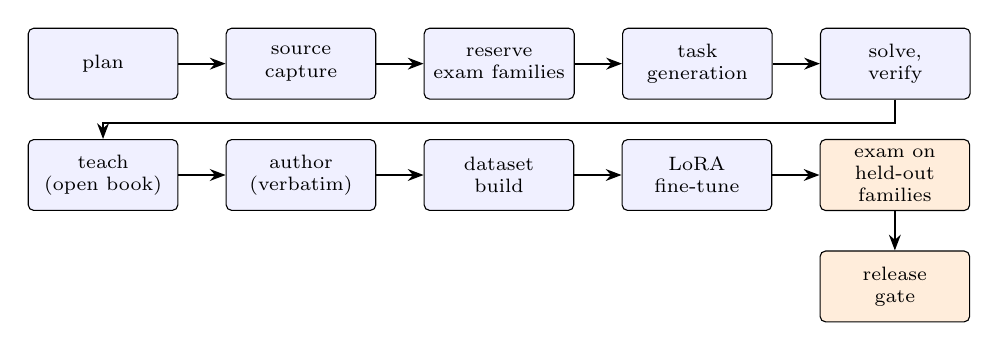
\begin{tikzpicture}[
  node distance=5mm and 6mm,
  box/.style={draw, rounded corners=2pt, minimum height=9mm, minimum width=19mm, align=center, font=\scriptsize, fill=blue!6},
  gate/.style={draw, rounded corners=2pt, minimum height=9mm, minimum width=19mm, align=center, font=\scriptsize, fill=orange!14},
  arr/.style={-{Stealth[length=2mm]}, thick}]
\node[box] (plan) {plan};
\node[box, right=of plan] (src) {source\\capture};
\node[box, right=of src] (res) {reserve\\exam families};
\node[box, right=of res] (tasks) {task\\generation};
\node[box, right=of tasks] (solve) {solve,\\verify};
\node[box, below=of plan] (teach) {teach\\(open book)};
\node[box, right=of teach] (author) {author\\(verbatim)};
\node[box, right=of author] (data) {dataset\\build};
\node[box, right=of data] (train) {LoRA\\fine-tune};
\node[gate, right=of train] (exam) {exam on\\held-out\\families};
\node[gate, below=of exam] (rel) {release\\gate};
\draw[arr] (plan) -- (src); \draw[arr] (src) -- (res); \draw[arr] (res) -- (tasks);
\draw[arr] (tasks) -- (solve);
\draw[arr] (solve.south) -- ++(0,-3mm) -| ($(plan.south)+(0,-3mm)$) -- (teach.north);
\draw[arr] (teach) -- (author); \draw[arr] (author) -- (data); \draw[arr] (data) -- (train);
\draw[arr] (train) -- (exam); \draw[arr] (exam) -- (rel);
\end{tikzpicture}}
\caption{The stages of one run, in order (the two orange stages measure). The reserve stage
precedes every generating stage, so no exam text is ever read by anything that makes
training data. Rehearsal and variant stages are omitted for clarity.}
\label{fig:pipeline}
\end{figure}

\paragraph{Models and hardware.}
Policy, teacher, task generator, planner and critic are all Qwen3-8B in non-thinking mode.
The judge is Qwen3-14B, a separate model loaded on its own. Two Tesla P40 cards (24~GB each)
are used, one job per card; the engine runs on them through Vulkan, and the policy base is
held in bf16.
Every job is launched through a wrapper that pins the card and stops the run if it
touches a CPU backend or software adapter, so a measurement can never silently come from
the wrong device.

\subsection{Stages}

\paragraph{Plan.}
A planner model reads a survey of the materials and chooses what to teach from a menu
of task kinds (recall, the author's own advice to a correspondent, explanation, conversation,
restoration of corrupted passages). Each choice is held to the survey by code: a kind
the sources cannot support is refused.

\paragraph{Source capture and reservation.}
The directory is captured as a source of text \emph{parts} (the Jefferson materials hold
1,629 parts; the Adams materials 307), split into sections that tasks cite by byte range.
Before any task is generated, the \emph{reserve} stage picks the families of the final test
and of a dev suite by a stable hash of the family name and removes the text of every edition
of each from every source later stages read (\cref{sec:split}).

\paragraph{Task generation.}
A generator model proposes tasks from sections; code admits or refuses each one. A task
must be grounded in its section, stand on its own without the source in front of the
student, name its subject, quote its source at a run of eight words rather than
paraphrase it, and not contradict another task. In the Jefferson run described below,
the generator was given 6,477~s and covered 19 of 1,629 parts; at that pace covering every
part would have taken 555,322~s, so only a sliver of the corpus is ever turned into tasks.
For the persona runs the generator is told the person wrote the sources.

\paragraph{Solve and verify.}
The policy attempts each task closed-book; tasks it always solves are dropped. A teacher
(here the same Qwen3-8B, shown the source passage) answers the rest open-book. Verifiers
are ranked by strength: executable checks, a \emph{stated} check that accepts an answer
stating the reference, an agreement check, and a calibrated judge. The strongest verdict
decides, and a judge alone never makes a training record. The student's training record
keeps the instruction and the verified answer but never the passage.

\paragraph{Author channel and variants.}
For a person, a second kind of record asks for a passage of the person's own text (at most 85
words) and keeps it only if a fit judge says the passage is a natural reply to the request.
Separately, the generator rewrites each kept task in other words; these \emph{variants} are
never trained on.

\paragraph{Dataset views.}
Records are projections of stored experience into training format. Three views matter here.
The \emph{dialogue} view holds verified teacher answers under the persona system prompt
(``You are Thomas Jefferson. Answer as Thomas Jefferson would: in the first person, in
Thomas Jefferson's own voice, from Thomas Jefferson's own experience and opinions. Answer the
user's request directly and concisely.''). The \emph{voice} view is built by code with no model
in the loop: the whole corpus of the author's text in chunks of 250 to 650 words, whole
sentences, closed at paragraph ends, one print of each text, no family over a tenth of the
tokens, half of them asked under the identity line instead of the persona prompt, each asked
for by a request built by code from its recipient, year and opening. In a later arm the
request is a 20--60 word description of the chunk's content written by the generator and
refused if more than 35\% of its words fall in runs of four or more words copied from the
passage. The
\emph{rehearsal} view holds the base model's own greedy answers to general tasks (sums and
format requests built by code with references, and general requests the base writes), kept
unless code decides them wrong. An optional abstention share trains the author to say the
writings do not settle a question; it is kept under half of the records, because a model
taught to stop that often stops answering.

\paragraph{Training.}
A candidate is a rank-8 LoRA adapter on all seven projections of every layer
(q, k, v, o, gate, up, down), trained by supervised fine-tuning in no-think mode
with loss only on the answer tokens and, in every run reported here, eight records per
step.
The current recipe is one learning rate for both entry commands (\code{train} and
\code{learn}, 2e-4), an alpha of twice the rank, no weight decay, AdamW with gradient
clipping at 1.0, a warmup of a twentieth of the steps, a cosine decay to a floor of a tenth
of the peak over the planned steps, and a step that is the mean over its supervised tokens,
with every record drawn once per epoch. A share of whole training families (a tenth of the
records, over at least three families where the data have them) is held back as a
\emph{monitoring} set scored at evaluations a sixteenth of the budget apart unless named
(every 15 steps for e4 and e1); the run keeps the adapter
of the best monitoring loss, and after four evaluations without improvement it lowers the
rate linearly to the floor over a tenth of the planned steps, still evaluating, and stops.
Of the candidates in \cref{sec:results}, e4 and e1 were trained with this recipe and all
others with the earlier one (\cref{sec:training-defects}).
Runs can keep the adapter of every evaluation so that a checkpoint may later be chosen on a
dev suite by generation quality rather than loss.

\paragraph{Exam and release gate.}
The exam (\cref{sec:eval}) measures whether the candidate generalises to held-out families.
The release gate has four checks: improvement over the champion on held-out and paraphrased
tasks (a sign test at $\alpha=0.05$), retention on earlier releases' tasks (bound 0.05),
a frozen \emph{anchor} suite of general tasks (110 items: 70 recall, 28 arithmetic, 12
format-following) with a drop bound of 0.02, and a serve check that plain \code{brain serve}
with the adapter gives the same answers on eight sampled tasks (at least 75\% agreement).
The improvement decision is the family-level sign test; task-level counts are reported
beside it. A release is an immutable adapter with a manifest of every number the gate
measured.

\subsection{Residency and memory on 24~GB cards}\label{sec:residency}

A bf16 Qwen3-8B occupies about 16.4~GB, and training at rank 8 with 1,024-token rows reached
a sampled peak of 21,407~MiB on one card. The 14B judge is a separate base that is not resident beside it. The
design consequence is that a device holds one base at a time and the work is staged so
that bases swap as seldom as possible: the policy, the candidate and the champion are one
base with different adapters attached before each generation (attached, never folded in,
because folding an adapter into a base forces a re-read of the checkpoint on every
switch); the gate and the exam answer \emph{every} task of a suite with every arm before the
judge loads; every resident base is released before a fine-tune or a \code{brain serve}
process loads its own copy; the serve check judges its answers only after the server has
exited; and the voice score loads one arm at a time and gives the device back between arms.
These rules came from failures: an out-of-memory fault on a card is not recoverable in
process (the engine reports a hard device fault and leaks the device rather than destroy
inconsistent driver state, so the run is lost), and in the earliest gate runs a judge that loaded while the server still held the
card ran out of memory, left every served answer ungraded, and the check counted ungraded
as ``different''. A served task with no answer is now ``not measured'', never a disagreement.

% SPDX-License-Identifier: CC-BY-4.0
% Copyright (c) 2026 Martin Schröder <info@swedishembedded.com>

\section{Evaluation Methodology}\label{sec:eval}

\subsection{What is estimated}

The decision-relevant quantity is the difference, on text the candidate and every
generator of its training data never saw, between the candidate asked under the prompt it is
deployed with and the \emph{base asked under the same prompt}. The unprompted base is
a secondary comparison. The distinction is not pedantic: in the first version of the
system every comparison against the base also changed the system prompt, so the effect of the
prompt was credited to the fine-tune. On the 31-task Jefferson exam the prompt alone moves the
base from 8 to 13 tasks judged right and its invented specifics from 21 to 6 (\cref{tab:exams}).
The exam therefore asks four arms the same tasks, each answered greedily (temperature 0,
at most 512 new tokens): the base under the default prompt, the base under the candidate's
persona prompt (\emph{prompted}), the candidate under the default prompt, and the candidate
under its persona prompt (\emph{deployed}). The primary comparison is fixed in the exam
manifest, before any model is put to it: deployed versus prompted, endpoint ``share of
tasks judged right on the greedy answer''.

\subsection{Family-level splits}\label{sec:split}

The corpora contain the same letters in several editions (about half of the letters of one
edition are printed in another). A split by file or by position therefore leaks: holding out
one print and training on another holds nothing out. The unit of every split is a
\emph{family}: texts that print the same text, in part or in whole, found as the transitive
closure of ``share at least eight distinct runs of eight words, wherever in either
text''. A run held by more than six texts is boilerplate (a formula of the period's
letters) and counts for nothing. The thresholds are set by what two unrelated texts can share by
idiom (a 12-word phrase is five runs and must not merge) against what a reused passage shares
(a 40-word passage is 33 runs).

Three defects in earlier versions of this rule are instructive, because each passed every
test that looked at the split itself:
\begin{itemize}
\item \textbf{A windowed comparison.} Texts were grouped by runs sampled from their first
  700 words. On 3,005 letters, comparing whole texts found 93 groups the windowed rule had
  left apart, 21 of them pairs sharing 50 or more distinct runs: letters printed by one edition
  inside a neighbour whose heading the parser had not cut at. Of the 1,625 files a run had
  been pointed at, 51 shared a passage of eight runs or more with a letter held out for the
  independent exam. Whole-text comparison of all 3,005 letters takes three seconds, so the
  window bought nothing.
\item \textbf{A parser that glued works into letters.} A letter ended only at the next
  letter's heading, so the last letter of a volume swallowed the works and appendices printed
  after it (one ``letter'' held 173,468 words, another 74,501). The overlap rule then
  merged them with thirteen letters, the \emph{Summary View}, the \emph{Manual} and the
  \emph{Notes on the State of Virginia} into one group of 16 files holding 419,188 of the
  1,553,235 words of the corpus (27\%): a group that can never be a meaningful held-out
  unit, and that made one of the monitoring families an outsized, non-letter text. A letter
  now ends at the first book, part, appendix or index heading, a stretch over 15,000 words
  is no letter, and the materials step refuses to write when an exam letter is one text with
  anything it would write.
\item \textbf{An exam that was not clear of the materials.} Of 413 families in the
  independent check, five had at least 90\% of their eight-word runs present in the
  training materials (and 44 had at least 5\%), because the glued ``letters'' carried them.
\end{itemize}

To remove the dependence on any rule being right after the fact, the exam's families are
\emph{reserved first}: a stable hash of the family name picks the families of the final
test and of the dev suite before any task is generated or dataset built, the text of every
edition of each is removed from every source that later stages read, and the exam tasks are
written from the reserved text alone. A candidate is never examined on a family it, or a
release it continues, was trained on. Every derivative record (a paraphrase, a description,
a verbatim passage, an abstention) inherits the family of its source and is confined to that
family's split.

\subsection{Tasks, answers and the judge}

Exam tasks are generated by the same admission rules as training tasks (grounded in the
reserved passage, self-contained, naming their subject). The reference for a task is the
source passage itself. Each answer is judged pointwise and blind to the arm: the judge
sees the task, the reference passage and the answer, and decodes greedily, so one answer
receives one verdict whenever it is judged, and no order among arms can reach a verdict.
The judge's prompt tells it to pass answers consistent with the reference, to fail answers that
contradict it, answer something else, dodge or only say they cannot tell, and to abstain
when it cannot decide; the judge's version number is bumped whenever its prompt, decoding or
parsing changes, so a calibration measured on another reading is not reused.

\paragraph{Calibration and controls.}
A judge is calibrated before its verdicts are read. The easy controls are each task's own
reference as the answer (must pass) and the reference of another family's task as the
answer (must fail). These only measure trivial cases, so the exam adds \emph{hard}
controls: each task answered with the reference of the task from another family whose reference
is closest in vocabulary, wrong by construction, so the share passed is the judge's
false-pass rate on a topical near miss. A judge with pass or fail precision below 0.9 is
untrusted and no claim is made. Qwen3-14B reached precision 1.0 on both on 48 easy controls in
every Jefferson exam; on the Adams exam pass precision was 1.0, fail precision 0.96, abstain
rate 0.02, with two controls misjudged. These are measurements on easy controls only. Agreement
with a person has not yet been measured (\cref{sec:limits}); the tooling exports a blind,
stratified sample (by arm, judge verdict and answer length) for a person to label and then
reports agreement, kappa, false-right and false-wrong rates and length bias.

\paragraph{Bias controls.}
Position bias is excluded by pointwise grading. Verbosity and self-preference
\citep{zheng2023judging,dubois2024lc} are handled less completely. The judge is told that
saying more than the reference is not a fault; length is otherwise not controlled except by
a \emph{like-length test}, which repeats the sign test on the tasks both arms answered within
a quarter of each other's length. The judge and the policy are both Qwen3, so
self-preference cannot be excluded. Deterministic checks override the judge wherever they apply: a recall
answer is decided by whether it states the reference, an executable task by running it, and
a separate code check marks an answer as having \emph{invented specifics} if it states a
number or more than one proper name that the task's source does not hold. This count is
reported beside the judged-right count because the judge is told to credit agreement with
the reference, not to detect extra claims. It partly measures verbosity, since a longer
answer states more specifics; answer lengths are recorded per arm so that this can be
examined.

\subsection{Statistics}

Tasks about one family are not independent, so the family is the unit of resampling. The
primary analysis pairs the arms by task: an exact one-sided sign test over the tasks only
one arm got right, reported with the difference in the share right and its 95\% percentile
bootstrap interval over families (10,000 resamples, seeded, each family contributing its own
tasks). The same test over families, each counted once by which arm got more of its tasks
right, is reported beside it; this is the test the release gate has always used. Secondary
comparisons (candidate under the default prompt, versus the unprompted base, and so on)
are corrected with Holm's step-down procedure~\citep{holm1979}; the primary comparison is
decided on its own. The report estimates the exam's own discordance and intraclass
correlation of the per-task difference (one-way analysis of variance estimator, floored at
zero) and the smallest true difference it could have shown, so that a null can be read as a
bound. Optional extra sampled answers per task give a continuous pass rate that is reported
beside, never in place of, the binary verdict.

\subsection{Power}\label{sec:power}

A family-level sign test needs a clean sweep. \Cref{fig:power} gives the exact power of
the two-sided test at $\alpha=0.05$ as a function of the number $n$ of discordant
families (those in which one arm got strictly more tasks right) and the probability $q$
that the better arm wins a discordant family. With six discordant families the test has
power \PowerSixNine\ even when the better arm wins 90\% of them, and \PowerSixEight\ at
80\%; reaching 80\% power at $q=0.8$ needs about 20 discordant families
(\PowerTwentyEight), and 40 give \PowerFortyEight. Our exams had between two and six
discordant families against the prompted base (\cref{tab:exams}). They could not have
succeeded unless every discordant family was a win and there were at least five of them
(one-sided) or six (two-sided).

\begin{figure}[t]
\centering
\begin{tikzpicture}
\begin{axis}[width=0.8\textwidth, height=6cm, xlabel={discordant families $n$},
  ylabel={power of the two-sided sign test}, xmin=1, xmax=60, ymin=0, ymax=1.02,
  legend pos=south east, legend style={font=\footnotesize}, grid=major, grid style={gray!25},
  tick label style={font=\footnotesize}, label style={font=\small}]
\addplot[thick, blue!60!black] table[x=n, y=q090, col sep=comma] {generated/sign_power.csv};
\addlegendentry{$q=0.9$}
\addplot[thick, green!50!black, dashed] table[x=n, y=q080, col sep=comma] {generated/sign_power.csv};
\addlegendentry{$q=0.8$}
\addplot[thick, orange!80!black, dashdotted] table[x=n, y=q070, col sep=comma] {generated/sign_power.csv};
\addlegendentry{$q=0.7$}
\addplot[thick, red!70!black, dotted] table[x=n, y=q060, col sep=comma] {generated/sign_power.csv};
\addlegendentry{$q=0.6$}
\draw[gray, thick] (axis cs:7,0) -- (axis cs:7,1.02) node[pos=0.5, right, font=\scriptsize, fill=white] {7 families};
\end{axis}
\end{tikzpicture}
\caption{Exact power of the family-level sign test ($\alpha=0.05$, two-sided) against the
number of discordant families $n$ and the per-family win probability $q$ of the better
arm. The vertical line marks the seven families of the pilot-scale exams.}
\label{fig:power}
\end{figure}

A task-level paired test is far more powerful, but its p-value depends on how the
discordant tasks split, which the stored marginals do not reveal. What the marginals do allow
is a bound: with $m$ net extra tasks right, the smallest one-sided exact sign p over all
possible splits is $0.5^m$ (\cref{tab:bounds}). Only the Adams exam (+8 net) could ever have
reached significance at the task level, ignoring clustering.

\paragraph{Sizing the final test by simulation.}
The planned test is the one the exam reports as primary: the deployed arm is better when
the lower end of the family-clustered bootstrap interval of the difference is above zero. We
simulate it: a task's difference is $+1$, $-1$ or $0$; a share \emph{discordance} of tasks
are $\pm1$; the first arm leads by \emph{effect}; and a family's mean difference is the
overall one plus a draw whose variance is the intraclass correlation (ICC) times a task's
variance. With no pilot estimate yet, we assume discordance 0.30 and ICC 0.10, so the
design effect is $1+(8-1)\times0.1=1.7$ for eight tasks per family.
\Cref{tab:power} gives the results. Two points matter. First, the planned 50 families of
eight tasks reach power 0.72, not the 0.8 an earlier estimate from the same assumptions suggested, for
a ten-point effect; it needs a fifteen-point effect to reach 0.97 and has power 0.23 at five
points. Second, the same simulation with 7 families of 5 tasks has a false-positive rate of
0.0725 at zero true effect: a percentile bootstrap over seven clusters is anti-conservative,
so even a nominally significant 7-family interval would deserve scepticism. These simulations
use 400 replicates and 500 bootstrap resamples, so each entry has a Monte Carlo error of about
$\pm0.02$.

\begin{table}[t]
\centering\small
\resizebox{\textwidth}{!}{\input{generated/power_table}}
\caption{Simulated power of the planned paired test (family-clustered bootstrap, lower bound
above zero), assuming a share of 0.30 of tasks discordant and an intraclass correlation of
0.10. ``Realised'' rows use the 39 families that yielded tasks and their mean of six tasks,
since 50 families were reserved but only 39 produced admitted tasks (244 tasks).}
\label{tab:power}
\end{table}

\paragraph{Procedure: pilot, simulate, freeze, open once.}
A pilot on the first 25 families by name (an arbitrary fixed order) estimates discordance and
ICC; the planned test is simulated with those; the size is frozen; a dev suite
(50 families of four tasks reserved beside the final test) chooses the checkpoint by a fixed
rule (at most 8\% invented specifics, then the best answers within a standard error, then
the loss on the dev families' own text); and the final test is run in full once, after one
checkpoint is chosen (the pilot's 25 families are a subset of it). The frozen exam is pinned by a ledger: the same name with other
content is refused, so every model is examined on the same tasks.

\subsection{Retention and the anchor suite}

The anchor suite guards against a persona fine-tune eroding general behaviour. It has 110
items graded by code. The gate computes the drop in accuracy of the candidate against the
base and fails when it exceeds 0.02. This test has two problems that no amount of
grading care removes. First, it is a point estimate on a paired binary outcome: with 17
discordant items the standard deviation of the paired drop under no change is
$\sqrt{17}/110=\AnchorSD$, so a bound of 0.02 sits about half a standard deviation from zero
and is exceeded in about 31\% of draws by chance. Second, to see a true two-point drop with
80\% power at the discordance observed (17 of 110, 0.155) the normal approximation
$n=(z_{\alpha/2}+z_\beta)^2 d/\delta^2$ gives about 3,000 paired items. The gate now
reports the paired bootstrap interval of the drop and the number of items needed beside the point
estimate; the 0.02 bound is unchanged because changing a bound is a change of rule, not a
report.

\begin{table}[t]
\centering\small
\resizebox{\textwidth}{!}{\input{generated/anchor_table}}
\caption{The anchor suite on three candidates. ``Drop'' is the base's accuracy minus the
candidate's; $p$ is the exact two-sided sign test on the discordant items. The bound is
0.02; the first two rows failed it, with $p=0.63$ and $p=0.45$.}
\label{tab:anchor}
\end{table}

% SPDX-License-Identifier: CC-BY-4.0
% Copyright (c) 2026 Martin Schröder <info@swedishembedded.com>

\section{Finding and Fixing Defects}\label{sec:defects}

The v7 run produced a candidate that passed the improvement check of the
release gate with a sign-test $p$ of $2.4\times10^{-4}$ and failed the anchor check by a
hair. Neither number meant what it appeared to mean. This section records how the
defects behind them were found, because the method is as reusable as the fixes.

\paragraph{Method.}
Four practices found nearly all of the defects.
\emph{(i) Read the code that makes the number, with file and line, before trusting the number.}
Two read-only audits (one of the pipeline's data and evaluation code, one of the training
engine) each produced a list in which every item cites the lines that establish it; claims
from a model-written report were treated as leads and checked in code or data.
\emph{(ii) Recompute the headline from its parts.} The gate's improvement figure was split
into the tasks it was made of; the anchor's drop was split into discordant items.
\emph{(iii) Diff the artefact against its input.} A prepared training file that is
byte-identical to its input exposed a rewrite that silently skipped every record
(a presence test where a non-empty test was meant). \emph{(iv) Treat the measuring
apparatus as under test.} Controls with a known answer, a rescoring of saved answers under a
corrected verifier, and a simulation of the test's own false-positive rate are all
measurements of the instrument.

\subsection{Defects of measurement}

\paragraph{The gate's ``held-out'' improvement was recall under paraphrase.}
The gate's improvement suite absorbed the \emph{variants}: paraphrases of tasks a trained
record was projected from. For the v7 candidate the suite called ``held-out'' held 149
tasks, of which 118 were variants and only 31 were truly held out. On it the candidate won
33 items against 3 (accuracy 0.408 against 0.204) and 12 of 12 discordant families,
$p=2.4\times10^{-4}$. The same candidate on the 31 genuinely held-out tasks won 2 of 2
discordant families against the unprompted base ($p=0.25$) and 2 of 3 against the prompted
base ($p=0.5$). Of the roughly 19 families that had any tasks only 7 were held out, so at
least 5 of the 12 winning ``families'' were training families. The check measures memory of
taught facts under paraphrase against the base under the \emph{default} prompt; it says
nothing about unseen letters or about beating the prompted base. The gate's report now keeps
generalisation to held-out records and recall under paraphrase apart, each with its own
difference, interval and sign test, and states the prompt each arm was asked each suite
under. The decision rule itself is unchanged.

\paragraph{A grader that failed correct long answers.}
Recall tasks were graded by a \emph{stated} verifier that accepts an answer stating the
reference, with a length bound of four times the reference's length plus 60 characters.
Because a verifier of formal strength outranks a judge, an answer such as
``There are seven continents: \ldots'' to a reference of ``seven'' was failed on length alone,
as were ``The hardest natural substance is \textbf{diamond}, \ldots'', ``H$_2$O'' against
``H2O'' (a subscript digit) and ``A spider has 8 legs.'' against ``eight''. In a separate
diagnostic run of the anchor suite, with both arms under the default prompt, the base
scored 0.800 and the v7 candidate 0.745 (10 candidate-only and 4 base-only misses); nine of
the ten candidate-only misses had the right content, and one was a real error. All nine
were long worked or explained answers, so the bug penalised the arm that gave them. The verifier now abstains on an over-long answer
that states the reference, leaving it to a judge, and reads sub- and superscript digits as
plain digits and whole numbers in words and digits as one.

Rescoring the saved answers of that diagnostic run with a reimplementation of the
corrected verifier (\cref{tab:rescore}) shows what remains. Under the corrected
verifier the candidate has 21 anchor answers waiting for a judge and the base 10. Counting
all pending answers wrong gives a drop of $+0.064$ (3 candidate-only against 10 base-only
items); counting them right gives $-0.036$ (5 against 1). On the 89 items decided by code for
both arms the candidate is at 0.955 and the base at 0.933 (drop $-0.0225$, 3 against 1, paired
bootstrap 95\% interval of the drop $[-0.067, 0.023]$). The sign of the drop therefore
depends on how a judge rules on 31 long answers. The reported ``forgetting'' was thus
partly a grading artefact; it was never a measured loss of knowledge.

\begin{table}[t]
\centering\small
\begin{tabular}{@{}lrrrr@{}}
\toprule
Arm & Right (old verifier) & Right (corrected) & Left to a judge & Wrong (corrected) \\
\midrule
Candidate (v7) & 82 & 85 & 21 & 4 \\
Base & 88 & 92 & 10 & 8 \\
\bottomrule
\end{tabular}
\caption{The 110 anchor items of the diagnostic run (both arms under the default prompt),
rescored under the corrected stated verifier.}
\label{tab:rescore}
\end{table}

\paragraph{A comparison that changed two things at once.}
Described in \cref{sec:eval}: the prompt moved the base from 8 to 13 of 31. The gate had the same
confound on the anchor, which it asked of the candidate under the persona prompt and of the base
under the default prompt, while the rehearsal records that were meant to protect general
behaviour were written under the default prompt. The anchor is now asked of both arms under
the default prompt.

\paragraph{A judge that was not calibrated on a hard case and not greedy.}
The calibration controls were the reference itself and an off-topic reference, so precision
1.0 on both said nothing about an on-topic answer that adds or contradicts specifics;
the powered exam adds \emph{hard controls} (\cref{sec:eval}). The judge decoded at
temperature 0.2 without a seed, so a verdict could change between two gradings of one
answer; it now decodes greedily. Five of the six exams of \cref{sec:results} were judged
before this change (\cref{sec:exam-versions}).
The judge and the policy remain the same model family (\cref{sec:threats}).

\paragraph{Per-task verdicts were never stored.}
The first exams stored only arm marginals and family-level tests. The per-task analysis that would
have shown whether the adapter beats the prompted base could not be redone: from the marginals
one can only compute the range of task-level $p$ that any split of discordant tasks would give
(\cref{tab:bounds,tab:prompt}). The powered exam stores every answer and verdict of every arm and
its analysis can be redone without a model. Its report is stored before the voice score
(which loads each arm on the device) so that a device failure there costs none of the exam.

\paragraph{A family-level test with seven units.}
The gate's held-out split was meant to reach at least eight groups (a quarter of the records,
newest first) but the quarter cap bound at seven families of 1, 4, 9, 2, 10, 4 and 1 tasks, because task
generation had covered only 19 of 1,629 parts. A family counts once whatever its size, so a
family of one task weighed as much as a family of ten.

\subsection{Defects of the training loop}\label{sec:training-defects}

The training engine's audit read the code and ran nothing. Its findings, with the correction
now in place (a mean over supervised tokens, epochs, annealing on stop and so on):

\begin{enumerate}
\item \textbf{Per-record loss normalisation.} Each micro-batch is one record, and loss and
  gradient were divided by that record's supervised-token count. Every record weighed equally
  whatever its length, so a 20-token answer's tokens weighed up to about ten times a 200-token
  answer's, and the printed training loss was a mean of per-record means, not comparable to
  the per-token held-out loss. The step is now a mean over its supervised tokens.
\item \textbf{The learning rate never annealed under early stopping.} Warmup was a fifth of
  the planned steps and the cosine ran over the plan; early stopping ended a run at step 56 of
  105 at a learning rate of $2.05\times10^{-4}$ against a peak of $3\times10^{-4}$.
  Warmup is now a twentieth of the steps, and a stop on patience is followed by a linear
  descent to the floor over a tenth of the planned steps, still selecting on every
  evaluation.
\item \textbf{Weight decay of 0.1 on the LoRA matrices.} Now 0 unless asked
  (\code{--weight-decay}). Whether it mattered is not established; with decoupled decay the
  total shrinkage over a run is at most about the product of rate, decay and steps,
  $3\times10^{-4}\times0.1\times105\approx0.3\%$.
\item \textbf{Alpha fixed at 16 at every rank.} Now twice the rank (\code{--alpha}). At
  rank 8 the two coincide, so every reported candidate, before and after the change, had
  alpha 16.
\item \textbf{Sampling with replacement.} Records were drawn uniformly with replacement and
  ``passes'' only sized the step budget. At 1.6 passes the expected share of records never drawn
  is $e^{-1.6}\approx20\%$. Records are now drawn in shuffled epochs, each once before any again.
\item \textbf{No packing.} Each record fills a row padded to the next power of two of the
  longest example; by the audit's estimate 70--85\% of the work was padding. This is not
  fixed; it limits throughput (about two minutes per step of eight records, including
  evaluation, for v7) and therefore the data a run can see.
\item \textbf{A learning rate defined twice.} \code{train} fell through to the engine's
  $3\times10^{-4}$ while \code{learn} used $2\times10^{-4}$, so the v6, ablation, v7 and
  rehearsal candidates (trained with \code{train}) had a peak of $3\times10^{-4}$ and the
  Adams candidate (trained inside \code{learn}) $2\times10^{-4}$. Both commands now share
  one value.
\item \textbf{A monitoring split that dropped records.} The monitoring set was one family (a
  group of 13 dialogue records and 57 voice records), so early stopping was decided on 25
  dialogue turns of a single family, and because the writer's text of a monitoring family
  was ``in neither file'', 57 of 210 voice records (27\%) never trained. The held-out,
  monitoring and training files now partition the records, the monitoring set spans at least
  three families where the data allow, and its loss includes the writer's text, which is most
  of the tokens.
\end{enumerate}

\paragraph{Multi-turn prefix stability.}
A chat template renders an earlier assistant answer without its reasoning block and the last
answer with it, so a single rendering of a whole dialogue cannot show every answer as it is
asked for, and its message boundaries are refused as not prefix-stable. A no-think
fine-tune therefore trains each supervised answer on the prompt the template renders for the
conversation so far, and on the completion the template renders after it (\code{answers\_as\_asked}),
one example per supervised answer, and fails loudly if the completion does not follow the prompt.
The rendering of training and evaluation must agree byte for byte: an earlier rewrite meant to
add the empty think block to training answers skipped every record that carried a \code{tools}
key, and every dataset wrote \code{"tools": []}. The trained file was byte-identical to its
input, which is how it was found; two runs of an earlier reasoning model had been scored
on a prefix they never trained on.

\subsection{Defects of the data}

\paragraph{The recipe starved the author's text.}
v7 trained 124 dialogue records (81 single-turn, 43 three-turn; about 29k supervised tokens
by a four-characters-per-token estimate) and 210 voice records (about 116k tokens) for
1.6 passes (448 record draws over 278 training records). All 210 voice records had the same user turn (``Write one of your writings, as you
wrote it.''); 7 were header-only (25--40 characters), 53 did not end at sentence punctuation,
43 did not start with a capital, 19 pairs shared five or more eight-word runs (duplicate
printings), and 157 sources supplied them with two sources supplying 23 and 18. The voice view was
rebuilt to cut the whole corpus into whole-sentence chunks with one print of each text, a cap per
family, and (optionally) model-written content descriptions as the request.

\paragraph{A quota that discarded a quarter of the answers.}
A cap per strength group applied once two groups existed; two recall answers created a
second, ``formal'', group and the cap discarded 39 of 163 judged dialogue answers (24\%). A
group under one candidate in twenty now counts for none of a dimension's groups.

\paragraph{A starved author channel.}
The fit judge for verbatim passages abstained on most items: 14 kept of 112 tasks (v7), 34
of 123 (v6), 52 of 171 (Adams). We report it as a limit on the amount of verbatim data the
dialogue pipeline can make; the voice view bypasses it.

\paragraph{Held-out text in training prompts.}
If passages are shown to the student (retrieval-style training), the library of passages was
built over all of the run's sources with no holdout filter. It is off by default and no
reported run used it; we list it because a split that holds for the data but not for the
prompts is a leak of the same kind.

\begin{table}[t]
\centering\small
\begin{tabular}{@{}>{\raggedright\arraybackslash}p{3.6cm}>{\raggedright\arraybackslash}p{4.6cm}>{\raggedright\arraybackslash}p{6.2cm}@{}}
\toprule
Defect & What exposed it & Measurement that proved it \\
\midrule
Gate improvement on paraphrases & Splitting the suite into its parts & 149 tasks = 31 held out + 118 variants; $p=0.25$ on the 31 \\
Stated verifier length bound & Reading the missed answers of the anchor & 9 of 10 candidate-only misses had the right content \\
Anchor cannot detect 0.02 & Counting discordant items & 17 discordant of 110; 7--10 split, $p=0.63$ \\
Windowed overlap rule & Comparing whole texts & 93 groups missed; 51 of 1,625 files shared a held-out passage \\
Glued ``letters'' & Looking at the largest group & 16 files, 419,188 of 1,553,235 words (27\%) \\
Monitoring dropped records & Simulating the split & 57 of 210 voice records never trained \\
Rewrite skipped all records & Diffing output against input & Trained file byte-identical to input \\
Per-record loss weights & Reading the loop & A short answer's tokens weigh up to $\sim10\times$ \\
Cap on strength groups & Reading the select log & 39 of 163 answers capped \\
Judge not greedy & Reading the judge's decoding & Temperature 0.2, no seed, in judge version 3 \\
\bottomrule
\end{tabular}
\caption{Defects, how each was exposed and the measurement that proved it.}
\label{tab:defects}
\end{table}

% SPDX-License-Identifier: CC-BY-4.0
% Copyright (c) 2026 Martin Schröder <info@swedishembedded.com>

\section{Results}\label{sec:results}

Every exam in this section is \textbf{pilot scale}: 31 to 42 tasks over 6 or 7 families. Their families are fixed by each run's held-out split before the candidate is trained,
but they are far too small to carry a claim, and
several candidates were selected against the same task sets (two exams share a 35-task set,
three share a 31-task set), so the comparisons are not independent. None is a frozen final test.
\Cref{sec:frozen} describes the powered exam that is.

\subsection{Candidates}

\Cref{tab:training} lists the training runs. The runs differ in more than the data (the
recipe changed between them, \cref{sec:training-defects}); we do not claim that any difference in
outcome is due to a single change. Held-out loss and token accuracy fall in every run, but token
accuracy is nearly flat (for v7 it moves from 0.731 to 0.750), which is expected for a stylistic
change~\citep{lin2024urial} and carries no information about voice. Losses are
not comparable across runs with different held-out sets.

\begin{table}[t]
\centering\small
\resizebox{\textwidth}{!}{\input{generated/training_table}}
\caption{Training runs. ``Step kept'' is the step of the adapter carried (``last'' for
unmonitored runs that carry the final step). v6 trained on dialogues only; ablation and v7 on
dialogues plus 210 fixed-prompt voice rows; e4 on dialogues plus template-prompted voice
chunks under the current recipe; e1 on dialogues plus the 210 fixed-prompt voice rows under the same recipe (not yet examined); adams on Adams dialogues plus voice rows. Peak learning rate
was not recorded for the earlier runs. Held-out records are scored with the base before
and the adapter after.}
\label{tab:training}
\end{table}

\begin{figure}[t]
\centering
\begin{tikzpicture}
\begin{groupplot}[group style={group size=2 by 1, horizontal sep=1.6cm}, width=0.48\textwidth,
  height=5.2cm, tick label style={font=\scriptsize}, label style={font=\small}, grid=major,
  grid style={gray!25}, legend style={font=\scriptsize}]
\nextgroupplot[xlabel={step}, ylabel={learning rate ($10^{-4}$)}, ymin=0, ymax=3.3, legend pos=south west]
\addplot[thick, red!70!black, mark=*, mark size=1.2pt] table[x=step, y expr=\thisrow{lr}*10000, col sep=comma] {generated/curve_v7.csv};
\addlegendentry{v7}
\addplot[thick, blue!60!black, mark=square*, mark size=1.2pt] table[x=step, y expr=\thisrow{lr}*10000, col sep=comma] {generated/curve_e4.csv};
\addlegendentry{e4}
\nextgroupplot[xlabel={step}, ylabel={monitoring loss}, ymin=0.85, ymax=1.3, legend pos=north east]
\addplot[thick, red!70!black, mark=*, mark size=1.2pt] table[x=step, y=monitor, col sep=comma] {generated/curve_v7.csv};
\addlegendentry{v7}
\addplot[thick, blue!60!black, mark=square*, mark size=1.2pt] table[x=step, y=monitor, col sep=comma] {generated/curve_e4.csv};
\addlegendentry{e4}
\end{groupplot}
\end{tikzpicture}
\caption{Learning rate and monitoring loss at each evaluation. v7 (recipe before the
corrections) stopped at step 56 of 105 with the rate still at $2.05\times10^{-4}$ and kept step
28; e4 (current recipe) annealed to $2\times10^{-5}$ and kept step 105. The monitoring sets
differ (v7: one family, dialogue records only; e4: several families including the writer's
text), so the levels are not comparable, only the shapes.}
\label{fig:curves}
\end{figure}

\subsection{Pilot-scale exams}

\Cref{tab:exams} gives, for each exam, the number of tasks judged right in each arm, the number
of invented-specifics answers, and the family-level sign test of the deployed candidate
against the unprompted and the prompted base. The $p$-values are one-sided exact tests
over discordant families, as the exam logged them.

\begin{table}[t]
\centering\scriptsize
\setlength{\tabcolsep}{3pt}
\resizebox{\textwidth}{!}{\input{generated/exams_table}}
\caption{Pilot-scale exams. ``Tasks/fam.'' is tasks over families; ``prompt.'' is the base under
the persona prompt; ``cand.'' is the candidate under the persona prompt; ``invented'' counts
answers that state a number or name absent from the source (of all tasks in the column).
Families are counted once whatever their size. v6 and ablation share one task set and v7,
rehearsal and e4 share another, so the pooled row, which sums the four rows v6, ablation,
v7 and adams, counts the first task set twice and is descriptive only.}
\label{tab:exams}
\end{table}

\begin{figure}[t]
\centering
\begin{tikzpicture}
\begin{axis}[ybar, width=\textwidth, height=5.8cm, bar width=7pt, ymin=0, ymax=0.7,
  ylabel={share of tasks judged right}, symbolic x coords={v6,ablation,v7,rehearsal,e4,adams},
  xtick=data, tick label style={font=\scriptsize}, label style={font=\small}, enlarge x limits=0.1,
  legend style={font=\scriptsize}, legend pos=north west, ymajorgrids=true,
  grid style={gray!25}]
\addplot[fill=gray!55] table[x=label, y=base, col sep=comma] {generated/arms.csv};
\addplot[fill=orange!70] table[x=label, y=prompted, col sep=comma] {generated/arms.csv};
\addplot[fill=blue!60!black] table[x=label, y=candidate, col sep=comma] {generated/arms.csv};
\legend{base, prompted base, candidate (persona prompt)}
\end{axis}
\end{tikzpicture}
\caption{Share of tasks judged right by arm in each pilot-scale exam (31 to 42 tasks each).
The prompt closes more of the gap than the fine-tune does; no panel has the power to resolve the
remaining difference.}
\label{fig:arms}
\end{figure}

The pattern is consistent but not conclusive.
\begin{itemize}
\item \textbf{The persona prompt does most of the work.} Pooled over the four exams
  (\PooledTasks\ tasks), the unprompted base is judged right on \PooledBase\ tasks
  (\PooledBasePct\%) and the prompted base on \PooledPrompted\ (\PooledPromptedPct\%): ten points
  from a prompt. The adapter is judged right on \PooledCand\ (\PooledCandPct\%), nine points
  above the prompted base.
\item \textbf{Invented specifics fall with the prompt and, a little, again with the
  adapter.} Pooled, the unprompted base invents on \PooledBaseInv\ answers, the prompted
  base on \PooledPromptedInv\ and the adapter on \PooledCandInv.
\item \textbf{No candidate separates from the prompted base.} The family-level test against
  the prompted base has $p\geq0.109$ in every exam. The best case, the ablation candidate
  (voice rows, 18 against 14 right), has five wins in six discordant families. The task-level
  bound (\cref{tab:bounds}) shows that the same exam could not have reached significance at the
  task level under any split of its discordant tasks, since only four net tasks separate the two
  arms.
\item \textbf{Against the unprompted base the evidence is stronger but still thin.} The
  ablation candidate won all five of its discordant families ($p=0.031$, one-sided; the test
  is on five units), the only family-level result below 0.05 in the table. Because the
  comparison is with an unprompted base, it does not separate what the prompt and what the
  adapter contribute.
\item \textbf{Adams is the largest difference.} 17 against 9 right with the prompted base
  (net $+8$ tasks) and 6 against 8 invented. At the task level the one-sided $p$ could lie
  anywhere from 0.004 to 0.084; at the family level, with six families and three discordant,
  the logged value is 0.125.
\item \textbf{Rehearsal and the new recipe do not change the picture.} The rehearsal candidate
  (v7 data plus replay of the base's own answers) judged 14 of 31 right against 13 for the
  prompted base; the e4 candidate 16 against 13, with 3 invented against 6 for the prompted
  base. Neither is distinguishable (family-level $p=0.5$ and $0.125$).
\end{itemize}

\begin{table}[t]
\centering\small
\input{generated/bounds_table}
\caption{What each exam's marginals allow: with $m$ net tasks in the candidate's favour over the
prompted base, the smallest one-sided exact task-level sign $p$ over every possible split of
discordant tasks is $0.5^m$ (ignoring family clustering, which only raises it).}
\label{tab:bounds}
\end{table}

\paragraph{The honest reading.}
The exams are consistent with an adapter that is a few points better than the prompted base
and with one that is no better. Pooled counts of tasks are descriptive, not a test: the
pooled task sets overlap, families are clustered, and the exams were used repeatedly to choose
recipes (\cref{sec:threats}). We therefore do \emph{not} claim that fine-tuning beats prompting
for this task. What the data do support is narrower: a prompt alone changes the answers
a good deal; a fine-tune that sees the author's text makes fewer unsupported specific claims
than the unprompted base (\PooledCandInv\ against \PooledBaseInv\ of \PooledTasks\ answers), and
is no worse than the prompted base on the measures we have.

\subsection{Release gate}

No Qwen3 candidate has been released. The Jefferson v7 candidate passed the improvement check
(subject to the defect above: 33 wins against 3, with 12 of 12 discordant families) and failed
the anchor check (accuracy 0.773 against 0.800, drop 0.027 against a bound of 0.02,
\cref{tab:anchor}); the serve check was not measured (\cref{sec:limits}). The Adams candidate
passed improvement (54 wins against 9 over 207 tasks, 165 of them variants; 13 of 13 discordant
families) and failed the anchor (0.764 against 0.800). The rehearsal candidate
passed the anchor (0.818 against 0.800, 9 candidate-only against 7 base-only items) but failed
improvement (29 wins against 7 items, but 8 of 11 discordant families, $p=0.113$) and the serve
check, which at that time counted ungraded served answers as different (\cref{sec:residency}).
A release was made once, for an earlier student model (a DeepSeek-R1 distilled 7B), where the
served model re-answered 8 of 8 sampled tasks alike. The rehearsal result is one run of one seed: it
does not show that rehearsal protects the anchor, because the anchor's own resolution is
only $\pm0.037$ (\cref{sec:power}).

\subsection{The frozen exam}\label{sec:frozen}

The final test and dev suite were reserved from the pool of letters left out of the materials,
before any task was generated. Fifty families were reserved for each. Generation admitted tasks
from only 39 families of the final test (244 tasks: 22 families with the full eight, the
others with one to seven) and from 44 of the dev suite (166 tasks), in the three kinds
conversation, advice and explanation. The planned 50$\times$8 design (400 tasks) was therefore
not reached. At the realised size the simulated power for a ten-point gain is 0.53 under the
planning assumptions (\cref{tab:power}). A 25-family pilot (155 tasks) is the first run on it; it
estimates the discordance and intraclass correlation that the simulation currently assumes.
\Cref{tab:pilot} lists the pilots. Runs that had not completed when this paper was written are
marked; they are not zeros, they were not measured.

\begin{table}[t]
\centering\small
\resizebox{\textwidth}{!}{\input{generated/pilot_table}}
\caption{Pilots on the frozen exam (deployed candidate against the prompted arm of the v7
pilot, paired by task, difference in points with the family-clustered 95\% interval). To update
a row, edit \code{data/pilot.csv} and rebuild.}
\label{tab:pilot}
\end{table}

\subsection{Cost}

Reported for planning, not as performance claims. Generating tasks over 19 of 1,629 parts took
6,477~s; teaching, verification, authoring, variants and selection for the v7 run took about five hours together
(257 teacher solves, of which 161 verified and 95 failed); training v7 took about two hours for 56
steps; an exam of 31 tasks over three arms with judging took about 38 minutes; a release gate
over 259 tasks and two arms took about two hours and 12 minutes. The first two figures are
the reason the pipeline cannot cover a corpus of this size with generated tasks (covering all
1,629 parts at the observed pace is 555,322~s) and the reason the voice view, which needs no
model, carries most of the author's text.

% SPDX-License-Identifier: CC-BY-4.0
% Copyright (c) 2026 Martin Schröder <info@swedishembedded.com>

\section{Discussion}\label{sec:discussion}

\paragraph{The exam, not the adapter, was the weakest link.}
The strongest conclusion from this work is about measurement. Every statistic the first
system produced was either uninformative (the anchor, whose bound sat inside its noise) or
about something other than the claim (the gate's improvement on paraphrases of trained
tasks, an effect of the prompt credited to the fine-tune). When those were corrected, the
remaining evidence on the adapter is a small positive difference over the prompted base with
an interval that, at the exam sizes available, includes zero. A power analysis would have
shown this before the first run: seven families, one vote each, cannot reject at
$\alpha=0.05$ unless every discordant family goes the same way and there are at least five of
them.

\paragraph{What the data support about the adapter.}
Three statements are supported. (i) A persona prompt alone raises the share of tasks judged
right and cuts invented specifics sharply (\cref{tab:exams}); a fine-tune must be compared
with it. (ii) Candidates trained on dialogues alone are indistinguishable from the prompted
base (v6: 14 against 14), which is what distilling a prompted teacher predicts
\citep{askell2021general}. (iii) The candidates that saw the author's own text word for word
are, in the pilot exams, never below the prompted base and above it by 1 to 8 tasks in all five
exams, a direction consistent with the closest comparable study
\citep{chakrabarty2025readers}; but the size is within what chance produces at
these sample sizes.

\paragraph{Why the voice view is the main lever, and why that is a hypothesis.}
Dialogues written by an 8B teacher under the persona prompt add little to what the prompt
already does. The author's own text is the only data that carries something the prompt cannot.
The first system gave this text little weight (210 fixed-prompt fragments, a loss that
favoured short teacher answers, a monitoring set that was dialogue only, a learning rate that
never decayed). Whether the corrected recipe with content-described chunks adds a measurable
amount is exactly what the pilots on the frozen exam are for; this paper does not claim
it.

\paragraph{Methodology that generalised.}
Four practices appeared repeatedly and are cheap: reserve the exam before generating
anything; fix the primary comparison before running it; store every per-task verdict so that
analyses can be redone offline and a power analysis can use the exam's own discordance; and
treat each instrument (judge, grader, split, bootstrap) as a thing to be measured, with
controls whose answer is known and a simulation of its false-positive rate.

\section{Threats to Validity}\label{sec:threats}

\paragraph{Construct validity.}
``Judged right'' means that a model judge says the answer gives what a source passage
says in reply to a generated task. That is a proxy for ``thinks like the author''; it rewards
knowledge of the passage and position, not prose style, and is silent on whether the reasoning is
the author's. A model that reads the exam's tasks and the passage would solve them, so the
tasks test the author's views as stated in the reserved letters. The invented-specifics
count is a code proxy for fabrication: it counts numbers and names absent from the source and
partly measures length.

\paragraph{Judge.}
Agreement with a person has not been measured; the judge was validated on controls only.
Judge and policy are the same model family, which invites self-preference that we cannot
exclude. The same family also wrote the tasks and the training data, so style and
topic distributions of exam and training tasks are related even though their source families
are disjoint.

\paragraph{Pretraining contamination.}
The letters are public domain and probably appear in the pretraining data of the base. The
exam is held out from fine-tuning, not from pretraining. Pretraining exposure would favour
all arms equally, including the prompted base, so it should not bias the primary comparison,
but it limits what ``held out'' means.

\paragraph{Adaptive reuse of the pilot exams.}
Recipes were developed over several runs examined on the same 31- and 35-task sets. Even if
an effect were observed there, selection on a small shared test set would overstate it. This is
the reason for the dev suite. The pilots on the frozen exam use its first 25 families by name, so
the final test is not unseen once they run; its analysis should report those 25 families and the
remaining ones separately.

\paragraph{Statistical validity.}
Seven-unit family-level tests have the power shown in \cref{fig:power}. A percentile
bootstrap over seven clusters is anti-conservative (false-positive rate 0.07 in simulation),
and we use it only on the larger exam. The power simulations assume discordance and ICC rather than
using values estimated from the data, and use 400 replicates. Pooled counts are descriptive only. There is one
training seed per recipe, so run-to-run variance of the adapter is unknown; one seed of the
v7 data has been trained (a second adapter) but not examined.

\paragraph{Internal validity.}
The recipe changed between candidates (data, learning rate, schedule, loss normalisation,
monitoring), so no pair of rows in \cref{tab:exams} isolates a single change. The earlier
candidates were trained at a learning rate (3e-4) different from the current default; v6,
ablation and adams did not record theirs.

\paragraph{External validity.}
Two authors, both eighteenth-century American, writing in English, whose corpora are large
(Jefferson) or modest (Adams), one base model, one adapter rank. Nothing here bears on other
languages, modern authors, or authors with little text.

\section{Limitations and Not Yet Established}\label{sec:limits}

\begin{itemize}
\item \textbf{No result on the frozen final test.} It has not been run in full. Pilots on its first 25
  families are listed in \cref{tab:pilot}; those not completed are not measured.
\item \textbf{No human labels.} Judge agreement, kappa, false-right and false-wrong rates and
  length bias on real answers are not measured. The tooling exists.
\item \textbf{Voice has no judge-free result.} The held-out text likelihood of each arm and
  the training-text overlap (8-, 13- and 20-word runs, longest shared run) are implemented but
  have no completed measurement. A fine-tuned model that quotes its training text is
  memorising, not thinking like the author; we cannot yet separate the two.
\item \textbf{No seeds.} A single seed per recipe; no estimate of run-to-run variance.
\item \textbf{The serve check was not measured} for any Qwen3 candidate: the serving binary
  was not available to the runs, and the check reports ``not measured'', never a pass.
\item \textbf{Retrieval is not evaluated.} The pipeline has retrieval-conditioned and
  abstention records and an exam arm with retrieved passages, but no measured run used them;
  all results are for a parametric model asked without retrieval. Retrieval itself was measured
  separately on 70 situations (semantic search found the source paragraph in the top ten for
  66\% of them, lexical for 30\%).
\item \textbf{Which correction mattered.} No training correction (token-normalised loss,
  annealing, weight decay, alpha, epochs) has been ablated. They are justified by audit and
  literature, not by an effect on the exam.
\item \textbf{Throughput.} Without packing, most of the compute on the P40s is padding, which
  bounds the data a run sees; a run over the whole corpus is expensive.
\item \textbf{Genuine ``thinking like'' cannot be proven.} The defensible claim is the
  observable one: on text excluded from training, positions, prose and abstentions are
  closer to the author's than the specified baselines'. We have not established that.
\end{itemize}

\section{Conclusion}

We built and examined a pipeline that learns from one sentence and an author's writings. Its
most useful products are methodological: a family-level split that survives overlapping
editions, an exam reserved before generation and sized by simulation, a judge with controls
and deterministic overrides, and a catalogue of defects that each changed a reported number.
Corrected, the evidence is that a persona prompt does much of the work, that no fine-tuned
candidate is statistically distinguishable from the prompted base at the sample sizes
measured, that the point estimates favour the adapters that saw the author's own text, and that
a properly powered test (39 families, 244 tasks) exists but has not yet been run in full. Until it is run, ``the adapter beats the prompt'' is a hypothesis.

% SPDX-License-Identifier: CC-BY-4.0
% Copyright (c) 2026 Martin Schröder <info@swedishembedded.com>

\section{Reproducibility}\label{sec:repro}

\paragraph{Data and models.}
The corpora are public-domain texts fetched by a checksummed script in the repository
(Washington, Randolph and Library editions of Jefferson's letters, his works, and an Adams
collection). The policy is Qwen3-8B (\code{BRAIN\_QWEN\_WEIGHTS} names the checkpoint, and
\code{SPLINTER\_BF16\_BASE=1} keeps the base in bf16) and the judge is Qwen3-14B, named as
\code{local:Qwen/Qwen3-14B@4096}. All models run locally.

\paragraph{Commands.}
The commands below are those the repository documents; every measured number in this paper
was produced by one of them or is derived from \code{data/} by \code{scripts/build\_data.py}.
\begin{small}
\begin{verbatim}
# materials for one person, and the pool an exam is reserved from
splinter-jefferson materials --resources RESOURCES --out ./materials
splinter-jefferson materials --exam-pool --resources RESOURCES --out ./pool
# the frozen anchor suite the release gate holds a candidate to
splinter eval --suite anchor --freeze samples/jefferson/anchor.jsonl \
  --freeze samples/adams/anchor-skills.jsonl
# one sentence, everything else autonomous
splinter "Learn to think like Thomas Jefferson based on the materials he has \
  written in directory ./materials"
# reserve and freeze an exam apart from any run (final test and dev suite)
splinter exam-set create ./pool --persona "Thomas Jefferson" \
  --families 50 --tasks-per-family 8 --dev-families 50 --dev-tasks-per-family 4 \
  --not-trained-by CANDIDATE
# size the exam by simulation, from an assumption or from a pilot report
splinter exam-set power --families 50 --tasks-per-family 8 --effect 0.10
splinter exam-set power --from-report PILOT.json --families 39 --tasks-per-family 6
# train, keeping the adapter of every evaluation; choose a step on the dev suite
splinter train DIALOGUES VOICE --steps 120 --records-per-step 8 --eval-every 15 \
  --keep-evaluations
splinter select CANDIDATE --exam-set DEV --judge local:Qwen/Qwen3-14B@4096 [--adopt]
# the powered exam: base, prompted base, candidate, candidate under persona prompt
splinter exam CANDIDATE --exam-set EXAM --resamples 1 [--pilot-families 25] \
  --judge local:Qwen/Qwen3-14B@4096 --prompt "to think like Thomas Jefferson" --json
# a candidate asked alone, to be paired offline with another report of the same exam
splinter exam CANDIDATE --exam-set EXAM --deployed-only ...
# analyses of a stored report; labels need a person
splinter exam-report labels-export REPORT
splinter exam-report labels-import LABELS
splinter exam-report memorisation REPORT
splinter release CANDIDATE --judge local:Qwen/Qwen3-14B@4096
\end{verbatim}
\end{small}
Every job in this paper ran through a wrapper that pins one card and stops on any CPU
or software-adapter line, one job per card.

\paragraph{Building this paper.}
\code{make} regenerates every table and plot data file from \code{data/} and builds
\code{paper.pdf}. To update a result, edit its row in \code{data/exams.csv},
\code{data/anchor.csv}, \code{data/training.csv}, \code{data/pilot.csv} or
\code{data/power\_simulation.csv}; the script recomputes the exact sign tests and refuses a row whose logged $p$
does not match the exact value.

\paragraph{Provenance of measured numbers.}
\Cref{tab:provenance} names the run log or report each number was read from.

\begin{table}[t]
\centering\small
\begin{tabular}{@{}p{4.5cm}p{9.5cm}@{}}
\toprule
Number & Source \\
\midrule
Pilot-scale exam counts and tests & Exam reports of each run: the Jefferson dialogue-only, ablation, v7, rehearsal and recipe-2 exams, and the Adams run's exam line \\
Gate improvement, anchor, serve & Release-gate reports of the v7, Adams and rehearsal candidates \\
Anchor rescoring & Saved anchor answers of base and candidate, rescored by a mirror of the corrected verifier \\
Training curves and held-out scores & Training reports of each run (step, learning rate, monitoring loss, held-out loss and token accuracy) \\
Stage timings, 19 of 1,629 parts & Task-stage summary of the v7 run \\
Peak device memory & Sampled device memory during v7 training \\
Frozen exam: 244 and 166 tasks & The exam manifests (tasks per family counted) \\
Power simulations & \code{splinter exam-set power} (400 replicates, 500 resamples, seed 0) \\
Exact sign-test power & \code{scripts/build\_data.py} \\
Per-task bounds & Computed from the marginals in \code{data/exams.csv} \\
\bottomrule
\end{tabular}
\caption{Where each measured number comes from.}
\label{tab:provenance}
\end{table}

\paragraph{Availability.}
Code, tests and this paper are in the Splinter repository; the sample READMEs list the
fetch and build commands for the corpora.


\bibliographystyle{plainnat}
\bibliography{references}

\end{document}
